\documentclass[oneside, german]{htwg-report}

% !TEX root = ../report.tex
% Use german umlaute
\usepackage{german,ngerman}
\usepackage[T1]{fontenc}
\usepackage[utf8]{inputenc}
\usepackage[ngerman]{babel}
\usepackage[autostyle=true,german=quotes]{csquotes}

%\usepackage[table]{xcolor}\usepackage{float}
%\usepackage{xcolor,colortbl}

\usepackage{epigraph}
\usepackage{float}
\usepackage{subfig}

\addbibresource{./bib/report.bib}

\begin{document}

\pagenumbering{gobble}

%% 'reporttype' add background elements to the cover / front page
%% possible values are:
%% bachelor	--> B S C
%% master	--> M S C
%% other		--> none
\reporttype{master}

\reporttypetext{Teamprojekt}

\newcommand{\verfasserA}{Lukas Hornung}
\newcommand{\verfasserB}{Lukas Luschin}
\newcommand{\verfasserC}{Moritz Schmidt}
\newcommand{\verfasserD}{Timmo Waller-Ehrat}
\newcommand{\verfasserE}{}
\newcommand{\thema}{Mehrbildkamerasystem zur räumlichen Detektion von Modellhubschraubern}
\newcommand{\hoschschule}{Hochschule für Technik, Wirtschaft und Gestaltung}
\newcommand{\institut}{HTWG Konstanz, Institut für Optische Systeme}
\newcommand{\prueferA}{Prof. Dr. Georg Umlauf}
\newcommand{\prueferB}{Prof. Dr Matthias O. Franz}
\newcommand{\prueferC}{Dennis Griesser}


\title[Mehrbildkamerasystem zur räumlichen Detektion von Modellhubschraubern]{\thema}

\doclocation{Konstanz}
\docdate{01. April 2018}

\makecover[]
%          
%% Include an optional title page.
%% !TEX root = report.tex
\begin{titlepage}
\newgeometry{hscale=0.81,vscale=0.8}

\AddToShipoutPicture*{\BackgroundImgTitelPage}

\vspace*{\bigskipamount}


%% Print the title in htwg-teal.
{\makeatletter
\fboxsep=0pt
\colorbox{htwg-white}{\begin{minipage}[t]{145mm}
    \begin{center}
        %% Print Report Type Text
        \color{black}\Huge{\@report@typetext}
        \\
        %% Print Report Title
        \color{black}\Huge\textbf{\@title}
    \end{center}
\end{minipage}}
\makeatother}

\bigskip
\bigskip

{
\setlength{\parskip}{0.5cm}
\begin{center}
	\textbf{zur Erlangung des akademischen Grades}
	
	\textbf{\Large \type\ of Science (\typeshortcut. Sc.)}
	
	\textbf{an der}
	
	\textsf{\huge Hochschule Konstanz}\\
	{\small Technik, Wirtschaft und Gestaltung}
	
    \textsf{\Large Fakultät Informatik} \\
	Studiengang \studiengang
	
\end{center}
}

\bigskip
\bigskip
\bigskip

\begin{center}
	\begingroup
	\renewcommand*{\arraystretch}{1}
	\rowcolors{2}{white}{white}
	{\makeatletter
		\begin{tabular}{lll}
			\type kandidat: & \verfasser \\
							& \strasse \\
							& \wohnort \\ \\ \\ \\
	
			1. Prüfer: & \prueferA \\
			2. Prüfer: & \prueferB \\ \\ \\ \\
			
			Ausgabedatum: & \ausgabedatum \\
			Abgabedatum: & \abgabedatum
		\end{tabular}
		\makeatother}
	\endgroup
\end{center}


%% reset page margins
\newgeometry{hscale=0.7,vscale=0.8}
\end{titlepage}




% !TEX root = report.tex
\chapter*{Extended Abstract}

\begin{center}
	\begingroup
	\renewcommand*{\arraystretch}{1}
	\rowcolors{2}{white}{white}
	{\makeatletter	
		\begin{tabular}{p{3.2cm}p{9.6cm}}
			Thema: & \thema \\
			& \\
			Teammitglieder: & \verfasserA, \verfasserB, 
			\verfasserC, \verfasserD\\
			& \\
			Betreuer: & \hoschschule \newline \institut \newline \prueferA, \prueferB \\
			& \\
		\end{tabular}
		
		\makeatother}
	\endgroup
\end{center}

\bigskip

\noindent
Unser Projekt behandelt das r"aumliche Detektieren eines Modellhubschraubers. Die Detektion soll unter Laborbedingungen, das hei"st, der Helikopter befindet sich vor einer wei"sen Wand, stattfinden. Mittels der Detektion soll auf einem Bild angezeigt werden, wo sich der Mittelpunkt des Helikopters befindet. Auch die Tiefe (Entfernung zur Kamera) des Helikopters soll ermittelt werden. F"ur diese Detektion sollen zwei oder mehr Kameras verwendet werden. Bei diesen handelt es sich um HIERKAMERAEINF"UGEN, die mit dem Computer "uber ein FireWire-Kabel verbunden sind.\newline

\begin{figure}[H]
	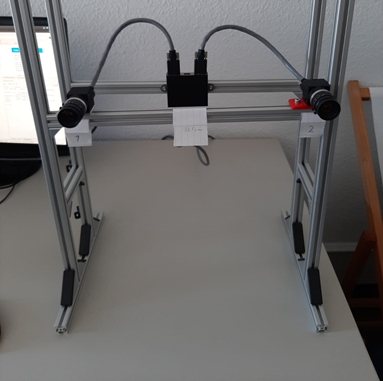
\includegraphics[scale=1.0]{bilder/camerasystem}
	\caption[Kamera-System]{Kamera-System}
\end{figure}

\noindent Das Projekt wurde erfolgreich umgesetzt.
Mittels zwei Kameras, die auf einer geraden Linie angebracht sind, kann der Mittelpunkt des Helikopters und dessen Abstand zur Kamera ermittelt werden.\newline
Unser Programm kalibriert als erstes die Kameras einzeln und anschlie"send zu einander. Das Kalibrieren erfolgt "uber ein Schachbrett-Muster. Sind die Kameras zueinander kalibriert, kann mittels eines Feature-Detektors eine Punktewolke des Helikopters generiert und der Mittelpunkt berechnet werden.

\begin{figure}%
	\centering
	\subfloat[Kamera-Kalibrierung]{{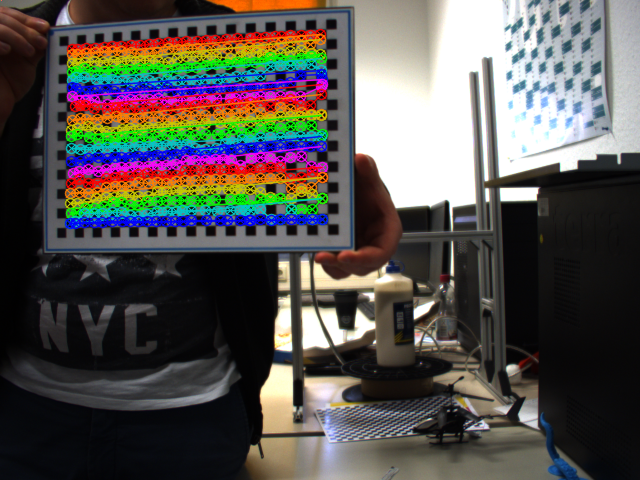
\includegraphics[width=6cm]{bilder/calibration} }}%
	\qquad
	\subfloat[Helikopter-Punktewolke]{{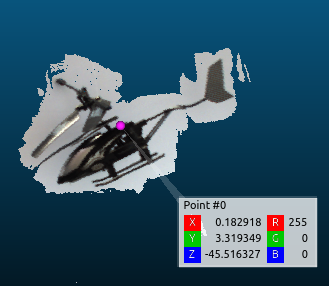
\includegraphics[width=6cm]{bilder/helicloud} }}%
	\caption{Kamera-Kalibrierung und Punktewolke}%
	\label{fig:example}%
\end{figure}
\noindent Eine m"ogliche Erweiterung des Projekts w"are das Kalibrieren von zwei Stereo-Systemen zu einander, um eine noch h"ohere Genauigkeit zu erlangen. Dies wurde versucht umzusetzen, ist allerdings gescheitert.



\tableofcontents
\newpage
\chapter{Einleitung}
\label{cha:einleitung}

\section{Aufgabenstellung und Zielsetzung}
\label {sec:aufgabenstellungzielsetzung}

Im Rahmen dieses Teamprojekts stand die Entwicklung eines Mehrbildkamerasystems zur r"aumlichen Detektion eines Modellhubschraubers. Dies beinhaltet sowohl das Erkennen des Helikopters, als auch die Abstandsmessung von diesem. Dies sollte mit Hilfe von Bilderverarbeitungs- und Machine Learning-Techniken, sowie der Verwendung von zwei oder mehr Kameras umgesetzt werden.\newline
Die Lernziele umfassten das Erlernen des Umgangs mit Kameras f"ur die industrielle Bildverarbeitung, sowie ein Verst"andnis f"ur die Grundlagen industrieller Signalverarbeitung zu schaffen. Zudem sollten grundlegende KI-Verfahren erlernt werden.

\newpage

\section{Motivation}
\label {sec:motivation}

\setlength\epigraphwidth{15cm}
\setlength\epigraphrule{0pt}

\epigraph{\textit{\glqq Computer vision, or the ability of artificially intelligent systems to see like humans, has been a subject of increasing interest and rigorous research for decades now.\grqq{}}}{--- \textup{}Naveen Joshi\cite{NJ}\\}

\noindent Das maschinelle Sehen gewinnt in den letzten Jahren immer mehr an Popularit"at. Sei es in der Forschung oder z.B. in der Spieleentwicklung f"ur Augmented Reality. Durch die steigende Relevanz in der Praxis wurde auch unser Interesse f"ur dieses Themengebiet geweckt. Es ist spannend zu verstehen, wie komplex die Dinge, die f"ur uns Menschen selbstverst"andlich erscheinen, wie zum Beispiel das r"aumliche Sehen, eigentlich sind.
Ein weiterer Anreiz f"ur das Projekt waren die verschiedenen angewandten Technologien. Wir alle interessieren uns sehr f"ur das Programmieren. Viel Erfahrung in der Programmiersprache Python hatte aber anfangs keines der Teammitglieder. Somit war das Erlernen dieser Sprache eine weitere Motivation.\newline
Auch die zum Gro"steil verwendete und weit verbreitete Bibliothek f"ur Computer Vision-Anwendungen in Python ''OpenCV'' hat das Interesse an dem Projekt geweckt.

\section{Aufbau}
\label {sec:aufbau}
Die Ausarbeitung des Teamprojekts besteht aus drei Teilen.\newline
Anfangs wird kurz auf die angewandten Technologien eingegangen.
Anschlie"send wird die eigentliche Umsetzung und das Vorgehen erl"autert. Zuletzt wird auf die aufgetretenen Probleme eingegangen und ein Fazit gezogen.

\input{Technologien}


\end{document}

